\documentclass[a4paper, 10pt]{article}        %\documentclass{} slides report proc book 
\usepackage[margin=1in]{geometry}
\usepackage[]{graphicx}
\usepackage{indentfirst}

\usepackage[hyperref]{xcolor}
\definecolor{teal}{RGB}{0, 128, 128}


\usepackage{hyperref, xcolor}
\hypersetup{
        colorlinks = true,
        allcolors={teal},
        linkcolor={teal}
       %urlcolor=[rgb]{0,128,128},
     }
%\title{Variants Statistics in Beacon}     
\title{Viral Beacon Statistics  part 2}  

\begin{document}
\date{}
\maketitle


\section{Stats on variants}


Statistics are calculated using \href{https://github.com/clauw87/virusbeacon/blob/raw_ideas/query_by_region_alias.pdf}{\texttt{Query by region -by names/aliases}} and \href{https://github.com/clauw87/virusbeacon/blob/raw_ideas/filters.pdf}{\texttt{Filters}}.\\

I would keep separate this by sequencing technology (platform): Illumina vs Nanopore (for now only Illumina) and of course fastq vs consensus (for now only fastq)

\begin{enumerate}
\item Number of genomic positions with variants: 28754/ Number of genomic positions: 29903 (96.15758\%)
\item Frequency of variants per position: fig \ref{fig:needle}
\item Number of variants per position: (3: 5769; 2: 11021; 1:11964) fig \ref{fig:needle}
% (also for Frequency (sampleMatchingCount), counts of unique sequences/haplotypes or counts of runs having them?)
   \begin{figure}[!htb]
     \centering
      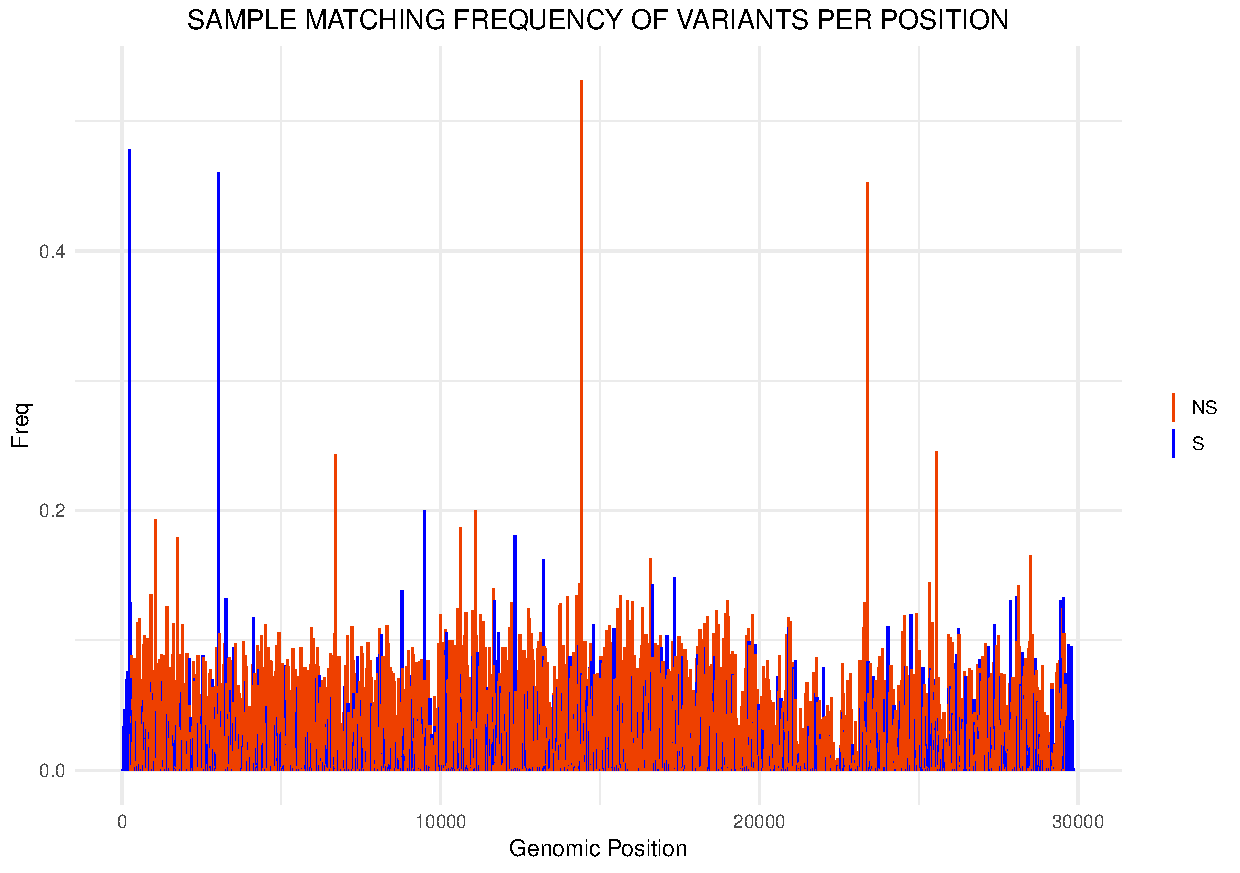
\includegraphics[width=0.8\textwidth]{needle.pdf}
       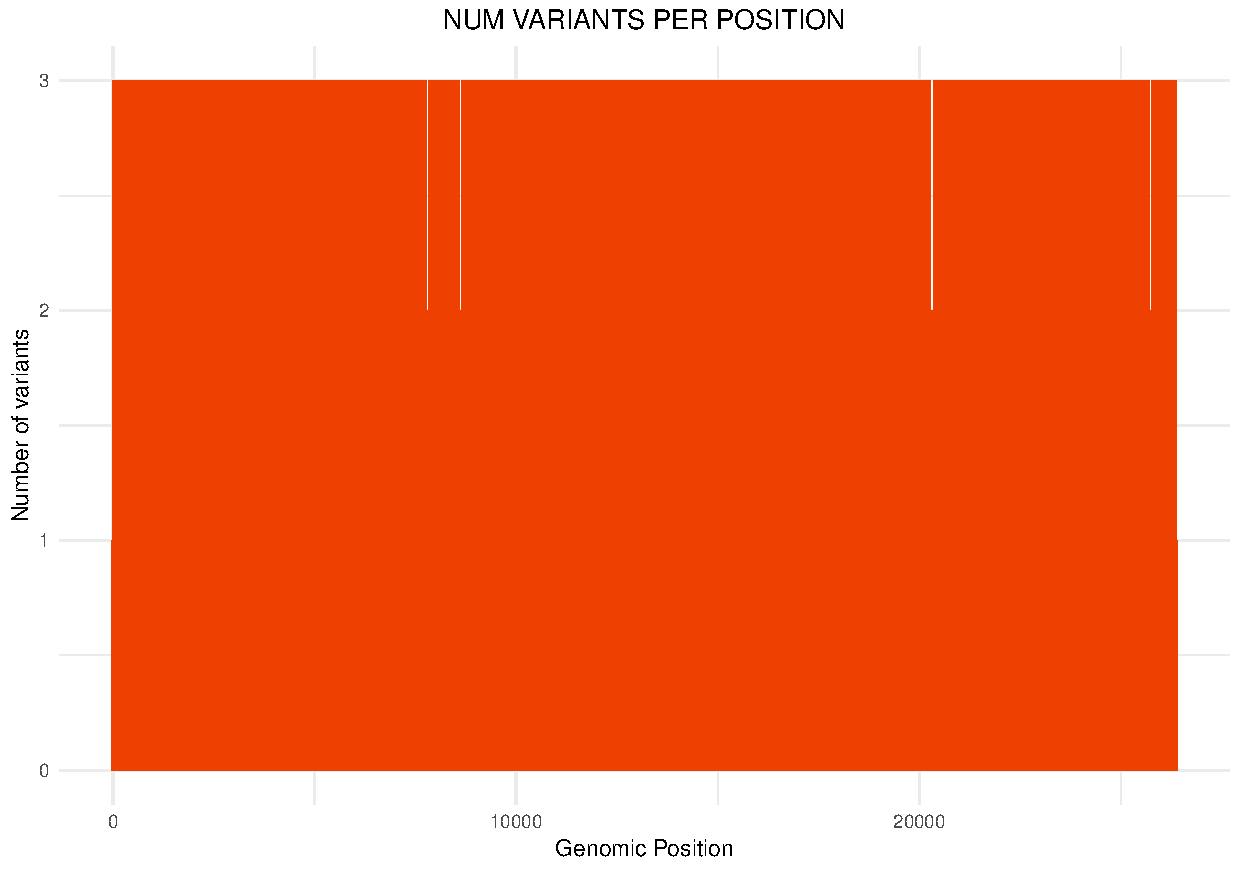
\includegraphics[width=0.8\textwidth]{needle_vpp.pdf}
       \includegraphics[width=0.7\textwidth]{genome_line.pdf}
      %\includegraphics[width=0.8\textwidth]{stats_menu1.pdf}
      %\includegraphics[width=0.8\textwidth]{beacon_stats_gp.pdf}
      %\includegraphics[width=0.8\textwidth]{beacon_stats1.pdf}
     %\includegraphics[width=1.2\textwidth]{stats1.pdf}
    %\includegraphics[width=0.7\textwidth]{gral_stats.pdf}
     \caption{Needle plot: Top: Frequency of variants per position. Bottom: Number of alternates per position}
     \label{fig:needle}
     \end{figure}
%\item[-] Unique Variant Frequency n terms of number of unique sequences/haplotypes having them/ sequences/haplotypes not having them\\
%\item[-] Variant Frequency in terms of number of runs having them/ runs not having them
\item Number of variants in database: 51313
\item Graph: Number of variants, split by options %, e.g fig \ref{fig:gral} 
\begin{itemize}
%\item[\textsl{option}] Split by sequence database: SRA, GISIAD, GWH
%\item[\textsl{option}] Split by geographic region: Australia, China, USA, Singapur, etc
%\item[\textsl{option}] Split by collection date (month)
\item[\textsl{option}] Split by variant frequency (groups) fig \ref{fig:freq}
     \begin{figure}[!h]
     \centering
     %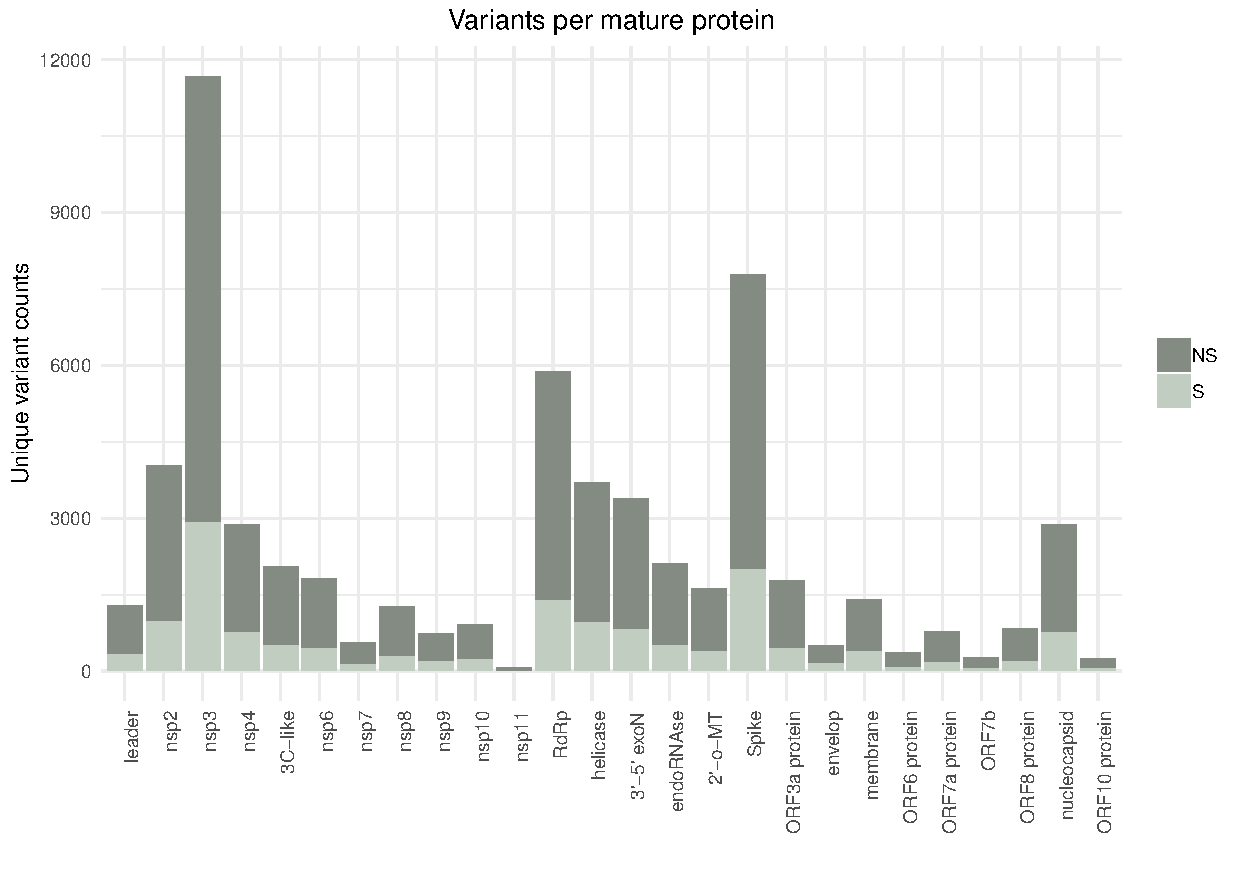
\includegraphics[width=0.8\textwidth]{variants_per_protein.pdf}
      \includegraphics[width=0.5\textwidth]{frequency.pdf} 
      %\includegraphics[width=1\textwidth]{by_protein.pdf}
  \caption{Number of variants per frequency group}
\label{fig:freq}
     \end{figure}
\item[\textsl{option}] Split by variant type field: SNP, indels (only SNPs) \colorbox{yellow}{Mau to check pipeline?} fig \ref{fig:gral}
\item[\textsl{option}] Split by genomic region: coding: all with genomic region=CODING, non-coding: the rest fig (further UTRs, intergenic?) fig \ref{fig:gral}
%\item[\textsl{option}] Split by variant effect: SYNONYMOUS CODING/ NON SYNONYMOUS CODING/ STOP GAINED, NON-CODING/ INTERGENIC, etc
\item[\textsl{option}] Split by molecular consequence (grouped: SYN: SILENT, NON-SYN: MISSENSE+NONSENSE, NONCODING:the rest) and further in all classes as in fig \ref{fig:gral} 

   \begin{figure}[!htb]
     \centering
     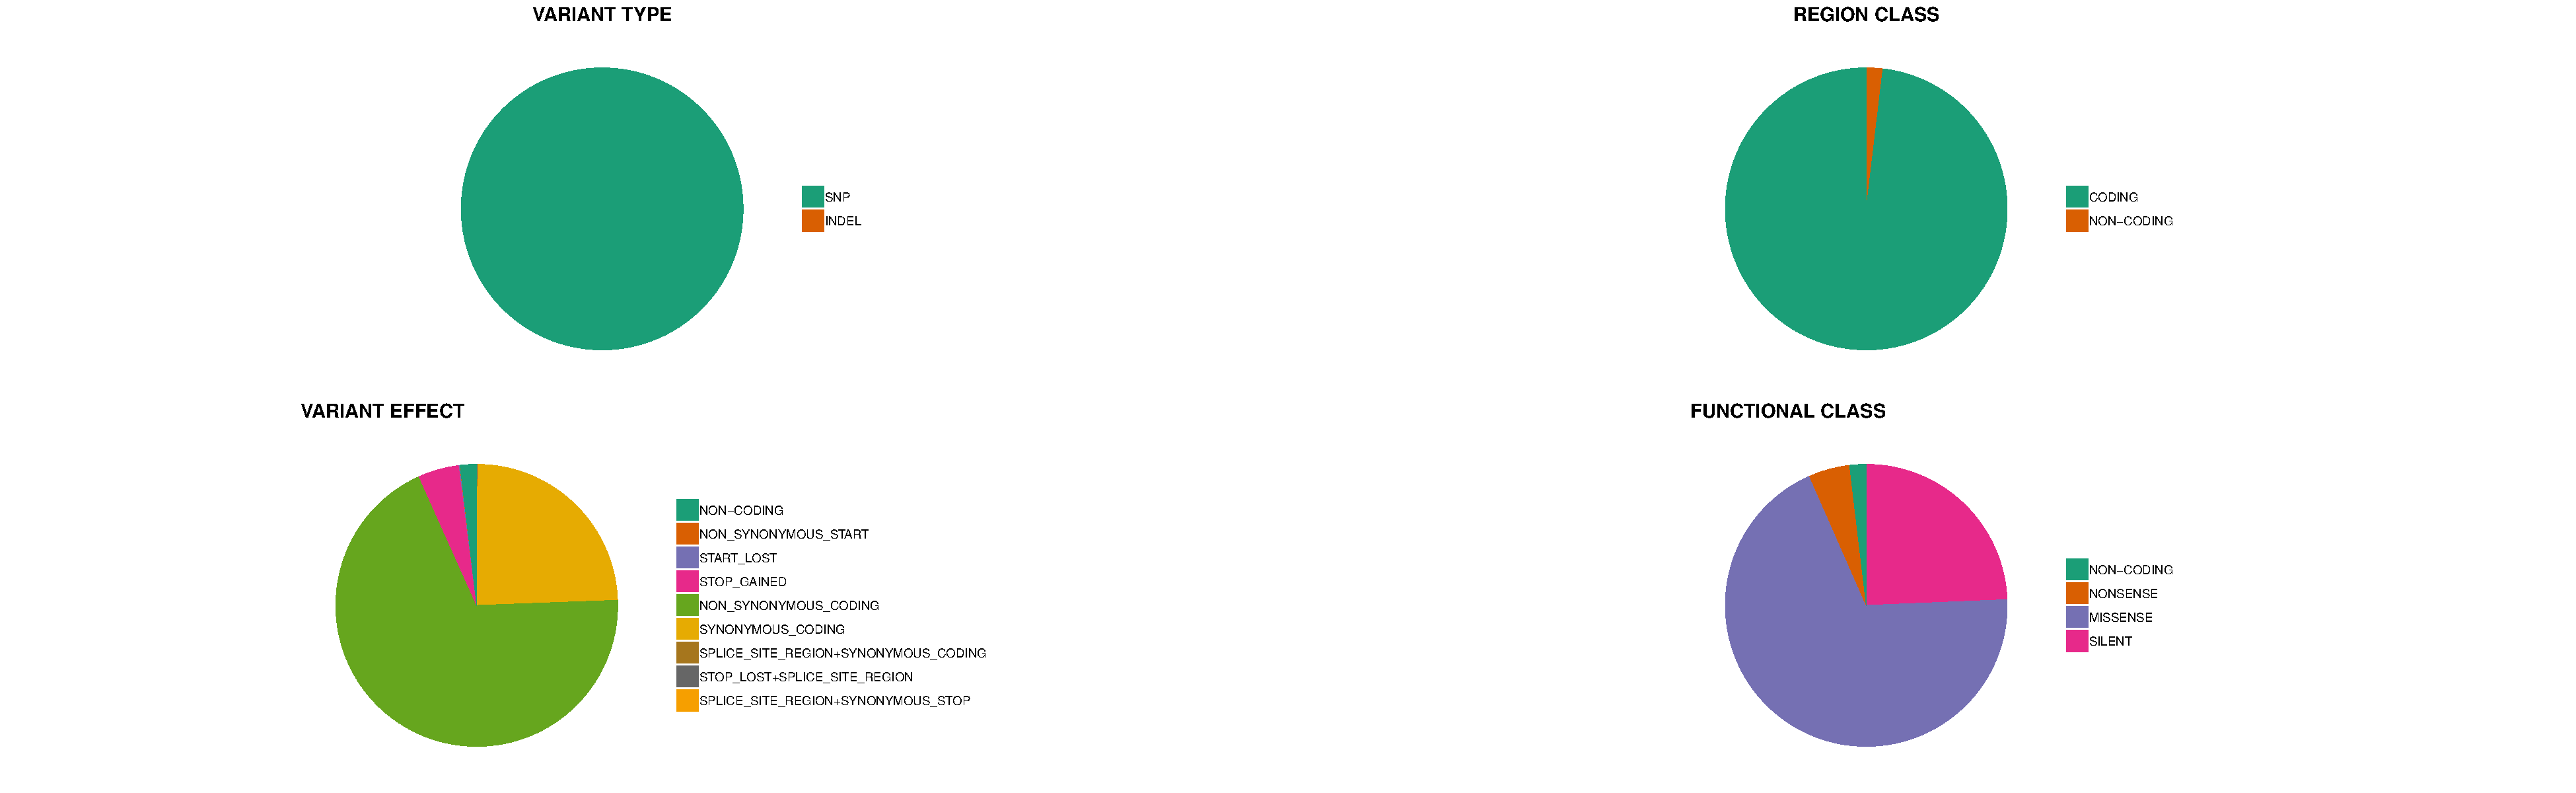
\includegraphics[width=1\textwidth]{variants_stats_all_pies.pdf}
      %\includegraphics[width=0.8\textwidth]{stats_menu1.pdf}
      %\includegraphics[width=0.8\textwidth]{beacon_stats_gp.pdf}
      %\includegraphics[width=0.8\textwidth]{beacon_stats1.pdf}
     %\includegraphics[width=1.2\textwidth]{stats1.pdf}
    %\includegraphics[width=0.7\textwidth]{gral_stats.pdf}
     \caption{Number of variants, split by variant type, region class, variant effect and mol consequence}
\label{fig:gral}
     \end{figure}
     
     
%\item[\textsl{option}] Split by Biosample sample.type
%\item[\textsl{option}] Split by Individual sex
%\item[\textsl{option}] See Per region Statistics: Distribution in genomic regions: \underline{non-coding}, \underline{gene}, \underline{cds/mature peptide}, \underline{stem loops}. Number of variants aggregated in regions, show also split by syn/non syn,  as in fig \ref{fig:mp}.
\item[\textsl{option}] See Per region Statistics: Distribution in genomic regions. Upon click on genomic region graph, expand to see per number of variants distribution in genomic regions: select \underline{NON-CODING}, and within \underline{CODING} show options: \underline{gene}, \underline{cds/mature peptide}. This will show individual components of each class fig  \ref{fig:genes} and \ref{fig:mp}.

\end{itemize}
%\item Number of positions with aminoacid changes in database/ Number of coding positions
\item Number of variants producing unique aminoacid substitutions in database: 18308
\item[\textsl{option}] Filter upon \underline{cds/mature peptide}. Number of variants producing aminoacid changes are aggregated in mature protein region
\item Number of unique aminoacid changes per protein \ref{fig:aa}
\end{enumerate}

     
        

%\subsubsection{Example Per region Statistics: Stats on variants distribution by \underline{cds/mature peptide} }

%I would make also stacked columns to show proportion of NON-SYN vs SYN in different colors. This would be based on field molecularConsequence in Variant Annotation. If molecularConsequence is SILENT, label as SYN, if it is either MISSENSE or NONSENSE label as NON-SYN.
%We could also present number unique aminoacid substitutions. 

%Although not the same info as in data from \href{http://cov-glue.cvr.gla.ac.uk/}{CoV-GLUE data (CVR Bioinformatics)}, since both synonymous and non-synonymous mutations data are included here (and unique variants are shown regardless of aminoacid change), the distribution looks pretty much the same, in agreement with what they say that selective pressure shifting non-synonymous/synonymous ratio hasn't been observed so far. Anyway, I would do the separated graph with non-synonymous variants.



\newpage


     \begin{figure}[!h]
     \centering
     %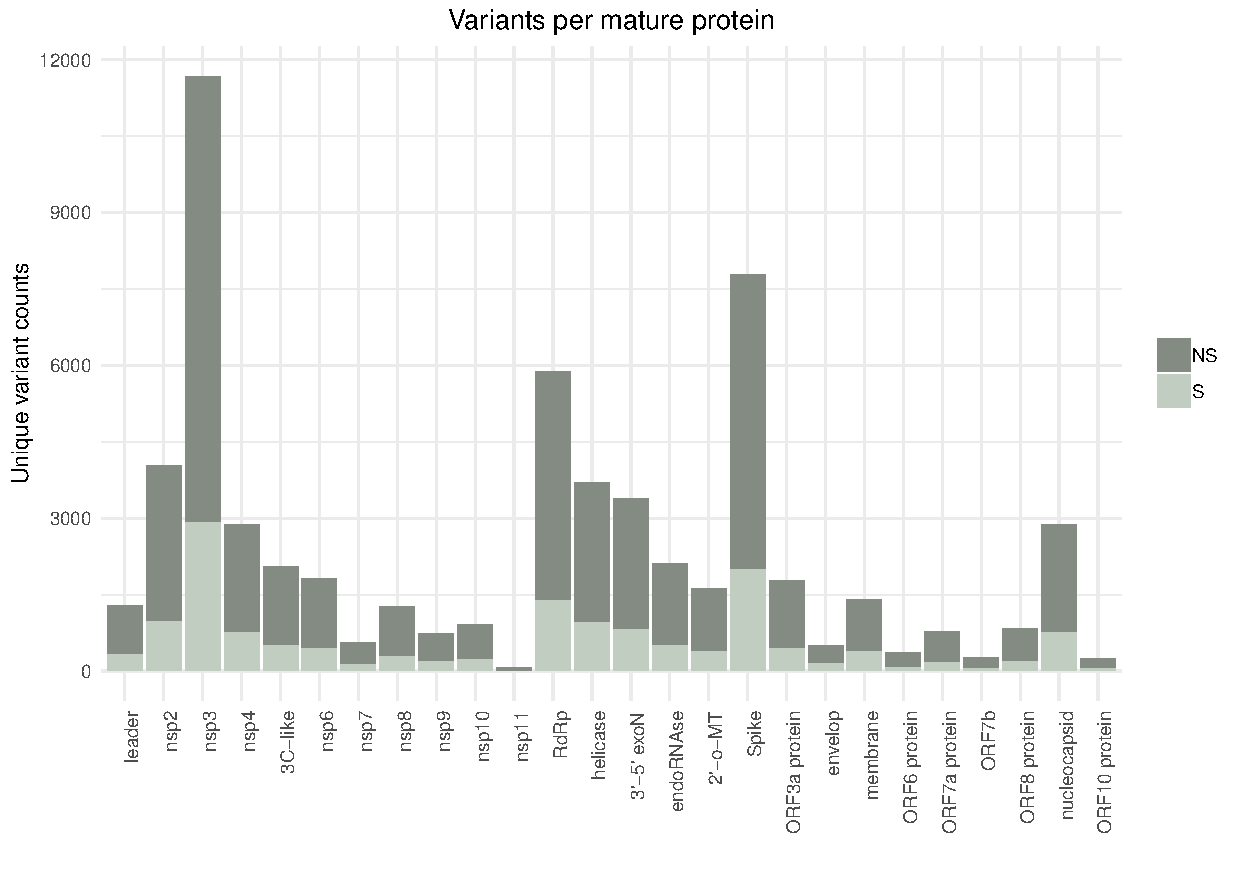
\includegraphics[width=0.8\textwidth]{variants_per_protein.pdf}
   \includegraphics[width=0.9\textwidth]{stats_menu_regions.pdf}
     % \includegraphics[width=1\textwidth]{by_protein.pdf}
            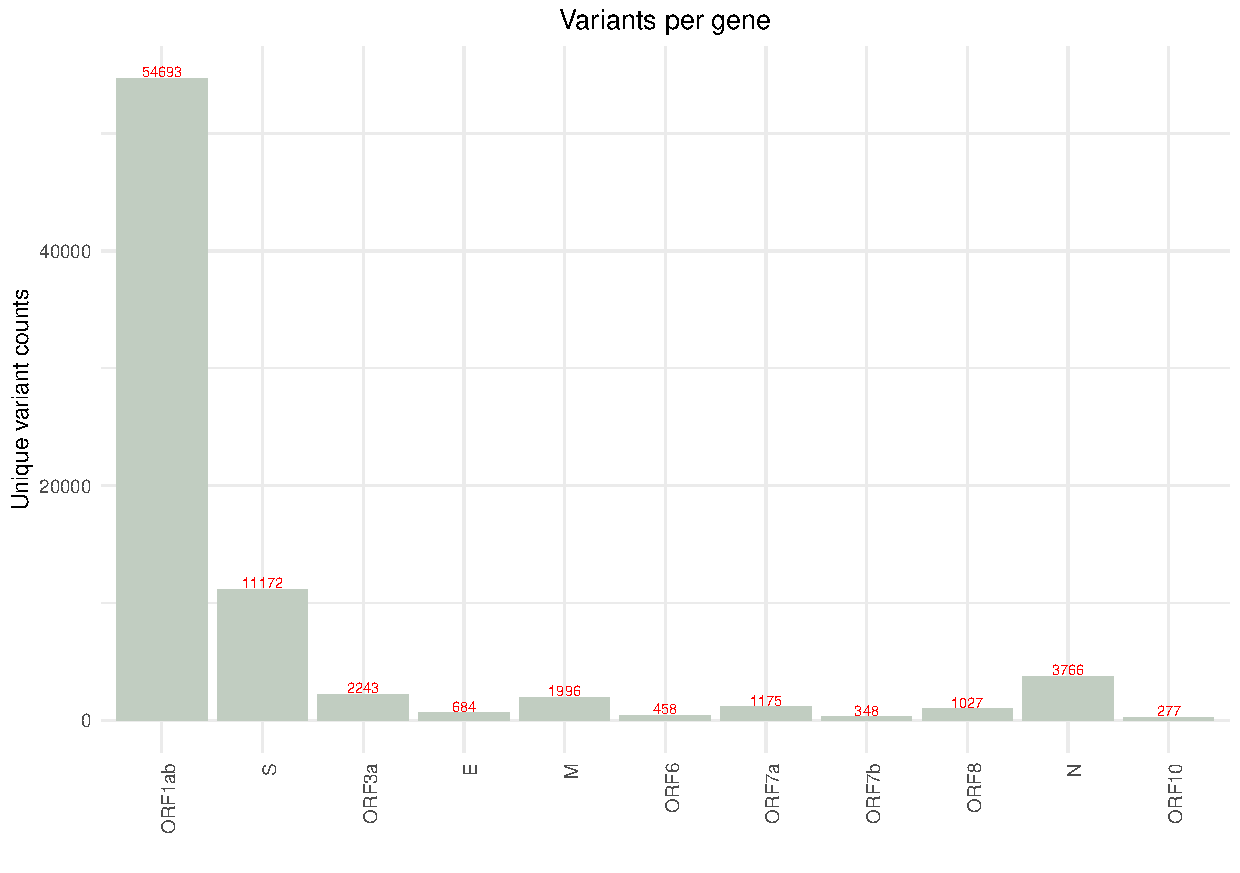
\includegraphics[width=1\textwidth]{variants_per_gene.pdf}
     \caption{Number of variants in coding regions of SARS-CoV2, shown per genes, shown directly  on clicking \underline{CODING area of genomic region graph} or in option "See variants distribution by region" {\color{blue}\underline{genes}}.
}
\label{fig:genes}
     \end{figure}






     \begin{figure}[!h]
     \centering
     %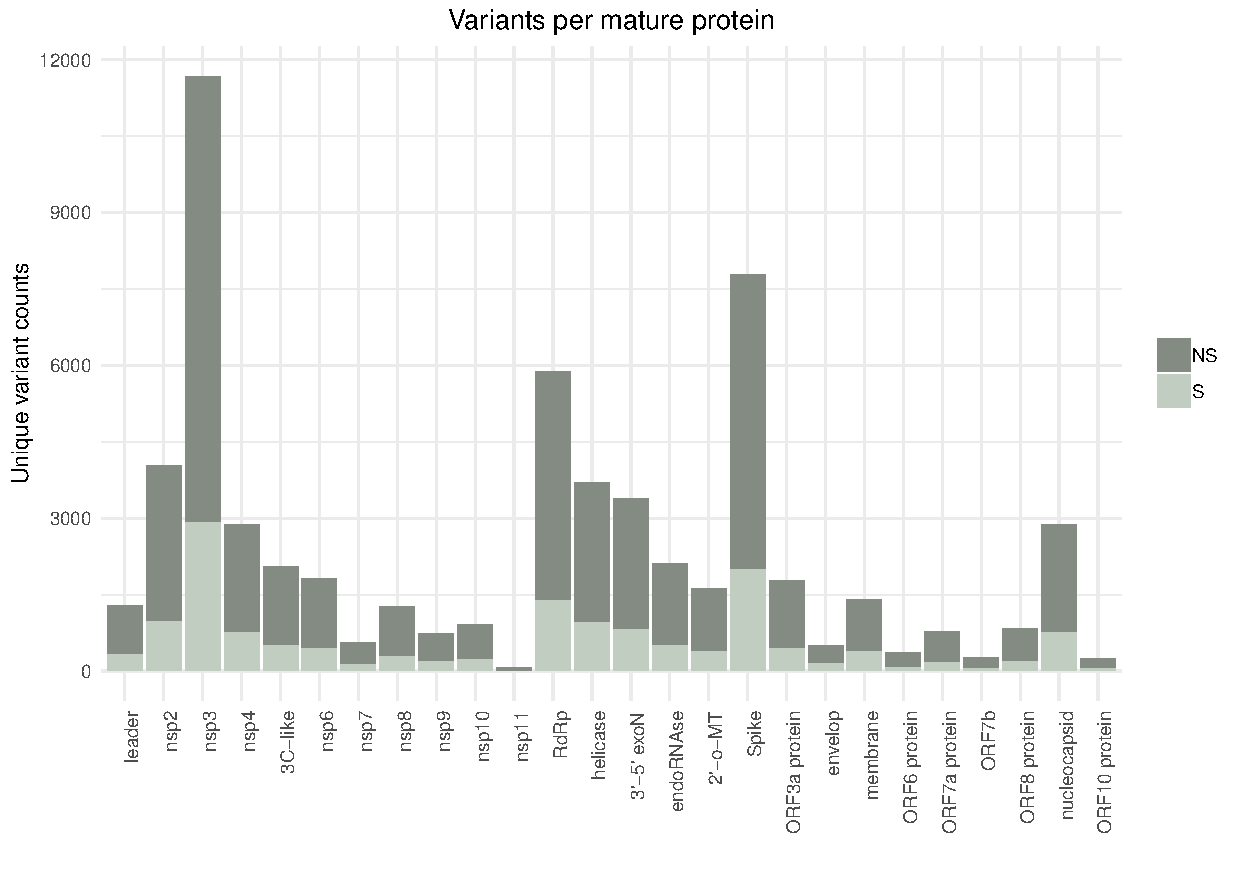
\includegraphics[width=0.8\textwidth]{variants_per_protein.pdf}
      \includegraphics[width=0.9\textwidth]{stats_menu_regions.pdf}
     % \includegraphics[width=1\textwidth]{by_protein.pdf}
            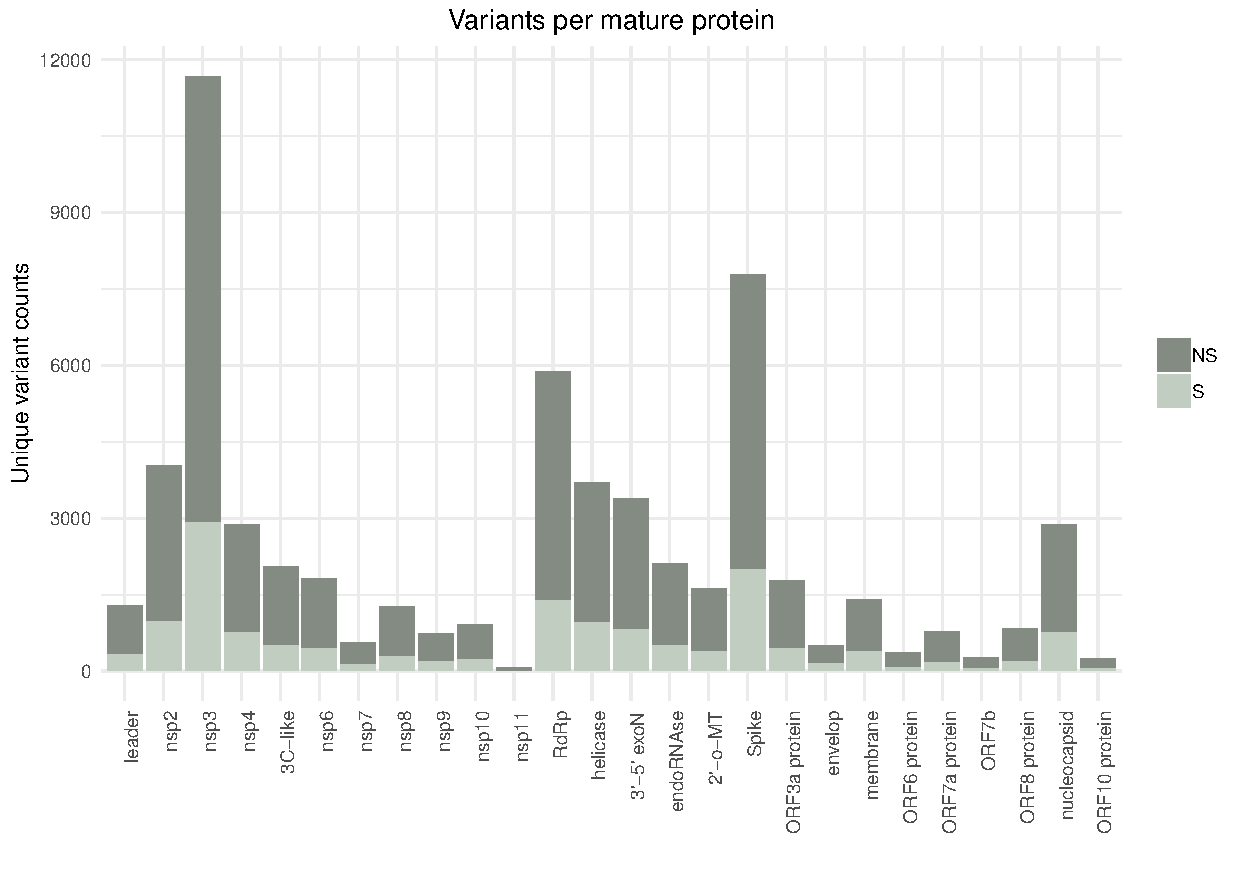
\includegraphics[width=1\textwidth]{variants_per_protein.pdf}
     \caption{Number of variants in coding regions of SARS-CoV2, shown per mature proteins,  split by split by syn/non-syn (dark green) shown on clicking \underline{cds/mature peptide} option within \underline{CODING area of genomic region graph} (which will show directly upon clicking the variants per gene graph \ref{fig:genes} or in option "See variants distribution by region" {\color{blue}\underline{cds/mat\_peptides}}. Options within this graph: \underline{split by syn/non-syn} (default in stack bar)  \underline{split by unique aminoacid changes}
}
\label{fig:mp}
     \end{figure}


     \begin{figure}[!h]
     \centering
     %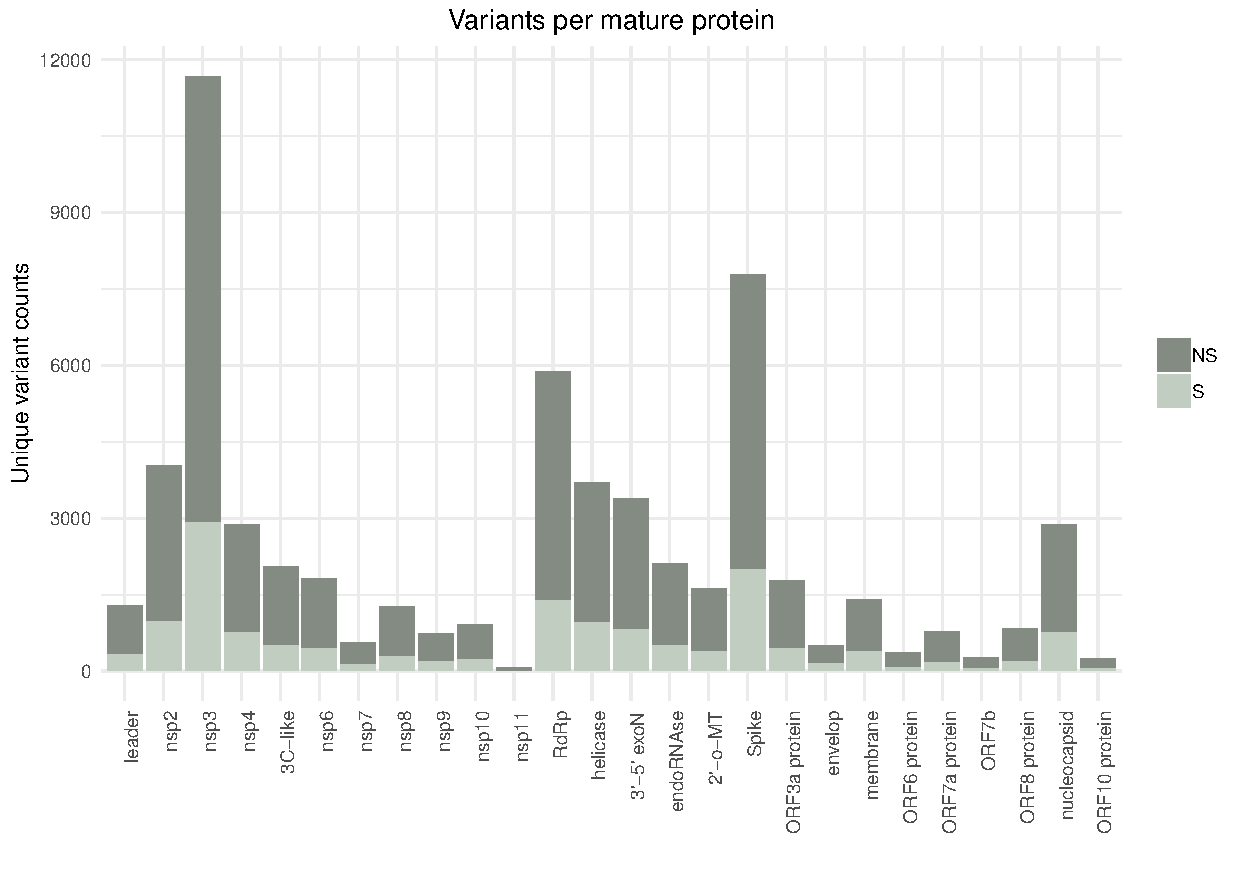
\includegraphics[width=0.8\textwidth]{variants_per_protein.pdf}
      \includegraphics[width=0.9\textwidth]{stats_menu_regions.pdf}
     % \includegraphics[width=1\textwidth]{by_protein.pdf}
            \includegraphics[width=1\textwidth]{aa_per_protein.pdf}
     \caption{Number of variants in coding regions of SARS-CoV2, shown per mature proteins, shown on clicking \underline{cds/mature peptide} option within \underline{CODING area of genomic region graph} (which will show directly upon clicking the variants per gene graph \ref{fig:genes} or in option "See variants distribution by region" {\color{blue}\underline{cds/mat\_peptides}}. Additional options within this graph: \underline{split by syn/non syn} (or default in stack bar)
}
\label{fig:aa}
     \end{figure}
     
     

%\subsection{Beacon data on mutations on non-coding regions}
%Figure \ref{fig:nc} shows non-coding regions such as UTRs and stem loops. Intergenic regions should be added as well.


    % \begin{figure}[!h]
   %  \centering
    %\includegraphics[width=0.8\textwidth]{variants_per_ncregion.pdf}
    % \caption{Unique variants in non-coding regions of SARS-CoV2. 5'UTR, stem loops (Coronavirus frameshifting stimulation element stem-loop 1, Coronavirus frameshifting stimulation element stem-loop 2, Coronavirus 3' UTR pseudoknot stem-loop 1, Coronavirus 3' UTR pseudoknot stem-loop 2, Coronavirus 3' stem-loop II-like motif (s2m), 3'UTR.}
  % \label{fig:nc}
     %\end{figure}



    \begin{figure}[!h]
     \centering
     %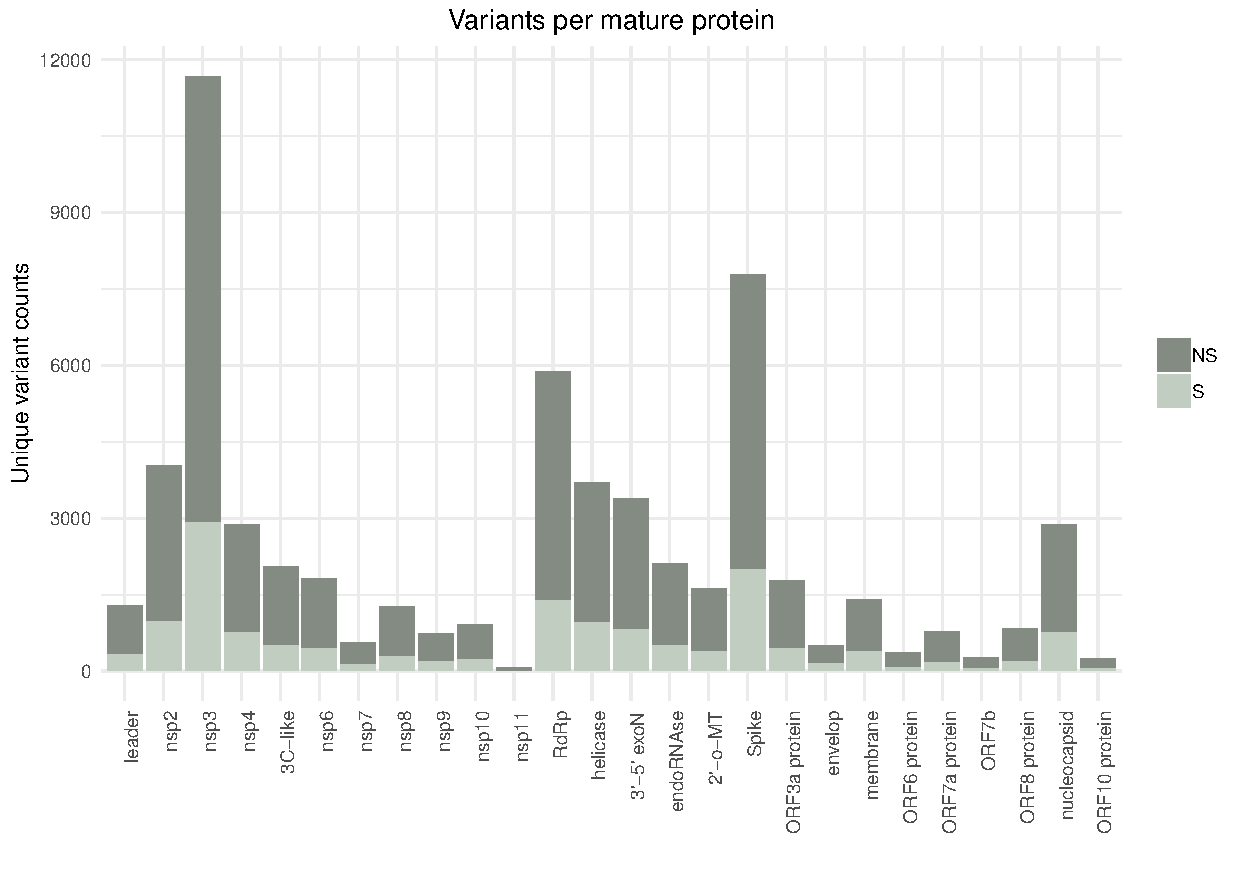
\includegraphics[width=0.8\textwidth]{variants_per_protein.pdf}
 \includegraphics[width=0.9\textwidth]{stats_menu_regions.pdf}
     % \includegraphics[width=1\textwidth]{by_protein.pdf}
            \includegraphics[width=1\textwidth]{variants_per_nc.pdf}
     \caption{Number of variants in non-coding regions of SARS-CoV2, shown per region, shown on clicking \underline{NON-CODING area of genomic region graph} or in option "See variants distribution by region" {\color{blue}\underline{noncoding}}.
}
\label{fig:nc}
     \end{figure}
     
     
     
         \begin{figure}[!h]
     \centering
     %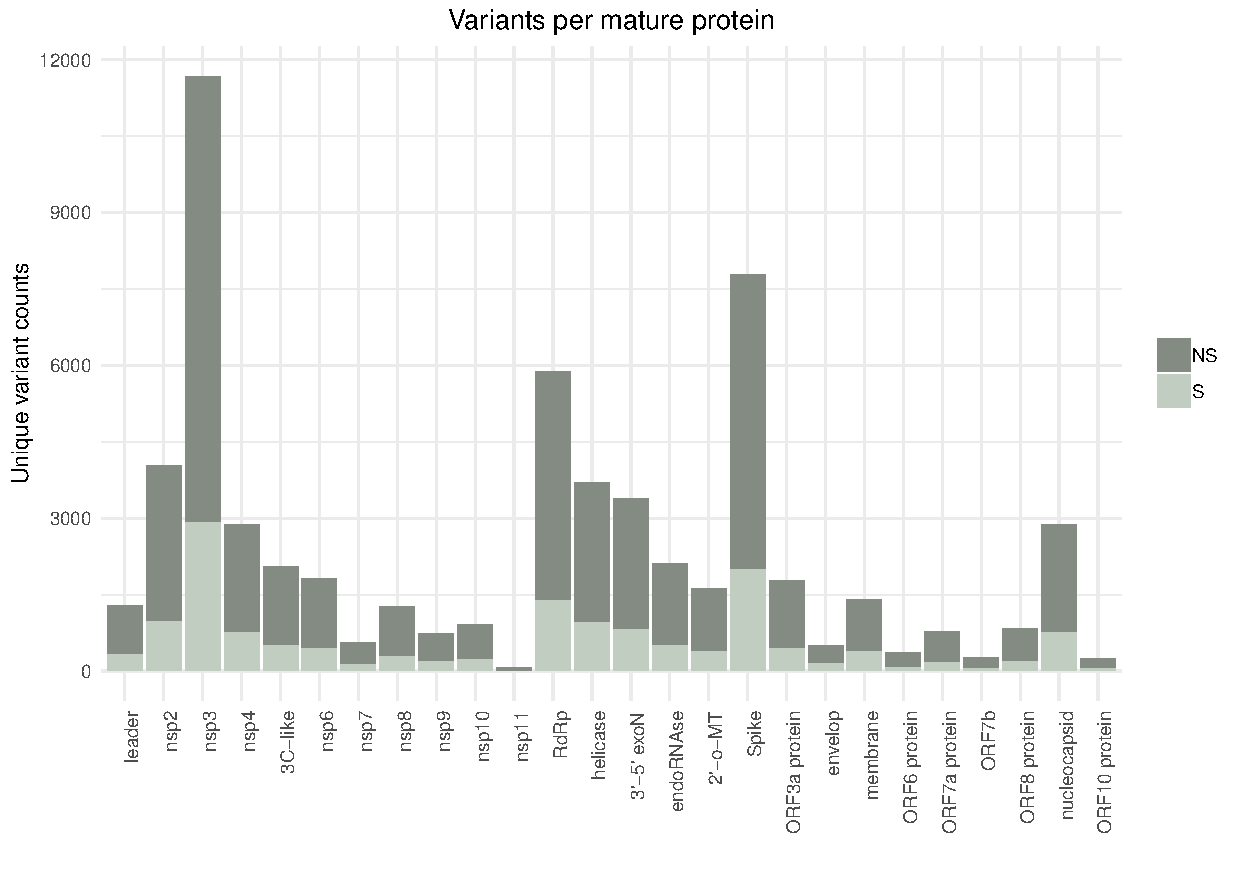
\includegraphics[width=0.8\textwidth]{variants_per_protein.pdf}
 \includegraphics[width=0.9\textwidth]{stats_menu_regions.pdf}
     % \includegraphics[width=1\textwidth]{by_protein.pdf}
            \includegraphics[width=1\textwidth]{variants_per_sl.pdf}
     \caption{Number of variants in stem loops regions of SARS-CoV2, shown per region, shown on clicking in option "See variants distribution by region" {\color{blue}\underline{stem loops}}.
}
\label{fig:sl}
     \end{figure}
     
     
     
     
     
     
\newpage
%On clicking on \underline{cds/mature peptide}, graph of the distribution of counts of unique mutations in coding regions grouped by mature proteins, split by syn/non syn, figure \ref{fig:mp}  \\




\end{document}













